\section{Resultados de la síntesis documental}
\subsection{CoAfina: alcance, productos y continuidad}
El informe de CoAfina 2023 registra 78 estudiantes, 16 equipos, 30 universidades y ocho países en una actividad virtual del 20 al 22 de octubre \cite{coafina}. La alianza organizadora incluyó LA-CoNGA physics, Creative Commons Venezuela, RedCLARA y CEDIA. El cuadro~\ref{tab:ediciones} separa ese recuento de las categorías necesarias para una comparación longitudinal. La convocatoria de 2024 identifica la tercera edición para el 19--21 de julio y comunica cerca de 150 estudiantes en ediciones anteriores; ese agregado no permite reconstruir inscripciones y finalización por año \cite{coafina2024}. La convocatoria archivada en el índice público para 2025 identifica una nueva edición, pero la página principal cambia con cada convocatoria \cite{coafina2025}.

\begin{table}[tbp]
\begin{threeparttable}
\caption{CoAfina por edición. Se conservan las unidades y los cortes temporales de cada fuente; una raya indica que no hay recuento documentado.}\label{tab:ediciones}
\input{build/ediciones-body}
\begin{tablenotes}[flushleft]
\item[a] Universidades de origen en el registro, no en la actividad final.
\item[b] 183 inscritos según la diapositiva de apertura de los organizadores (S1); corte de apertura, no actividad final ni registro individual depurado.
\item Actividad en 2022: aproximadamente la mitad de los inscritos; en 2023 y 2024, participantes reportados. En 2025 los siete retos corresponden a la apertura. Fuentes: \cite{coafina2022,coafina2023pre,coafina,uis2023,coafina2024,coafina2025,coafina2025apertura}.
\end{tablenotes}
\end{threeparttable}
\end{table}


La noticia de LA-CoNGA sobre 2023 enlaza demostraciones de soluciones y documenta el retorno de un participante de la edición anterior como proponente de un reto \cite{coafinacontinuidad}. Este es un ejemplo concreto de cambio de función dentro de la red. Las demostraciones conservan una explicación del producto; para verificar su ejecución futura se necesita además código, datos, dependencias y permisos. El hallazgo organizativo es que visibilidad del resultado y preservación ejecutable son tareas distintas, aunque ambas puedan formar parte de una misma entrega.

\subsection{Edición colaborativa con la OMS y Cornell}
El editatón de noviembre de 2021 conectó a OMS, Cornell, Wikimedia y Creative Commons. Su publicación de 2026 registra 45 inscritos de 12 países, 19 editores activos y 22 artículos nuevos; Creative Commons Venezuela aportó identidad visual y sitio bilingüe \cite{salud}. El artículo informa del reconocimiento concedido al equipo en 2022 por el Director General de la OMS en el desafío OMS LEAD 2021. La distinción reconoce la iniciativa; sus productos se identifican mediante ediciones.

Para el seguimiento, ALAN indica 2022; el boletín de Cornell anuncia ``Editathon V2: Health for All'' para el 13--16 de febrero de 2023 \cite{cornell}. Se mantienen separados ambos registros y se emplean únicamente las métricas de 2021 en la comparación.

Wikipedia aporta historial público y revisión posterior como parte de su plataforma. La literatura sobre su uso en salud destaca la importancia de participación experta y calidad de las fuentes \cite{wikihealth}. Para el diseño de un editatón esto implica preparar conjuntamente contenido y acompañamiento editorial: el conocimiento temático necesita traducirse a una contribución que la comunidad pueda revisar y mantener.

\subsection{Datos de física y reconocimiento académico}
El relato institucional de ATLAS documenta uso de datos abiertos en tesis venezolanas y acompañamiento a distancia \cite{atlas}. La tesis proporciona una pregunta sostenida, tutoría y reconocimiento académico; la posibilidad de reutilizar el análisis depende de los materiales que se conserven junto a la memoria. El caso permite identificar una vía institucional de continuación sin reducir todas las actividades abiertas a encuentros breves.

La conferencia de OpenGLAM de abril de 2020 sobre datos de ATLAS y competencias informáticas constituye otro punto de encuentro entre comunidades científicas y culturales \cite{openglam}. En formación de software, HSF e IRIS-HEP distinguen funciones de instrucción, mentoría y facilitación \cite{hsftraining}. Ambas experiencias ayudan a distribuir responsabilidades: quien propone el problema, quien acompaña su resolución y quien conserva el producto no tienen que ser la misma persona.

\subsection{Preservación, reconocimiento y continuación}
La figura~\ref{fig:modelo} resume la lectura transversal. Los formatos ofrecen apoyos diferentes: la plataforma editorial mantiene revisiones, la institución académica reconoce una trayectoria y el hackatón conecta retos con equipos. La decisión transferible es asignar explícitamente la función que el formato no garantiza por sí solo.
\begin{figure}[htbp]\centering
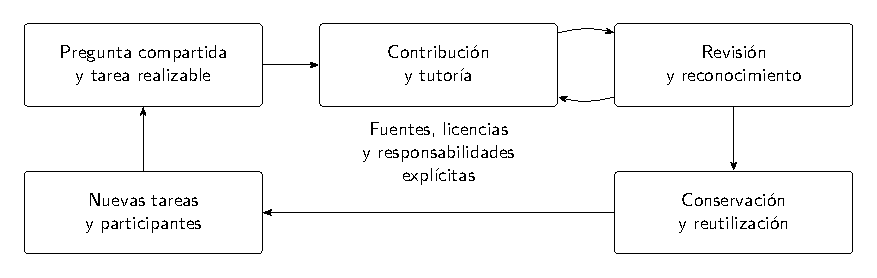
\includegraphics[width=160mm]{figures/modelo.pdf}
\caption{Matriz interpretativa de los casos. La última columna propone comprobaciones de continuidad; no representa tasas observadas de reutilización.}\label{fig:modelo}
\end{figure}
